\section{Experimental Evaluation}
\label{sec:exp}

{\bf Experimental environment.} All experiments in this section were
conducted on an 8-slave elastic cloud cluster using Linux Ubuntu 14.04
and Spark v1.4.  Each node had 4 cores and 16 GB of memory.  Spark
Standalone cluster manager and Hadoop 2.6 were used.

Because Spark is a lazy evaluation system, a \insql{materialize}
operation was appended to the end of each query, which consisted of
the count of nodes and edges.  In cases where the goal was to evaluate
a specific operation in isolation, we used warm start which consisted
of materializing the graph upon load.  Each experiment was conducted 3
times, we report the average running time and the measure of
variability.

{\bf Data and evaluation methods.}  We evaluate performance of our
framework on three real open-source datasets.  

\begin{enumerate}

\item DBLP\footnote{\url{dblp.uni-trier.de/xml}} contains
  co-authorship information from 1936 through 2015, with over 1.5
  million author nodes and over 6 million undirected co-authorship
  edges.  Total data size: 205 MB.

\item nGrams\footnote{\url{storage.googleapis.com/books/ngrams/books/datasetsv2.html}}
  contains word co-occurrence information from 1520 through 2008, with
  over 1.5 million word nodes and over 65 million undirected
  co-occurrence edges.  Total data size: 50 GB. \vera{verify}

\item
  DELIS\footnote{\url{law.di.unimi.it/webdata/uk-union-2006-06-2007-05}}
  contains monthly snapshots, from 05/2006 through 05/2007, of a
  portion of the Web graph focusing on the .uk domains, with a total
  of over 133 million nodes and over 5.5 billion directed
  edges~\cite{BSVLTAG}.  Total data size: 1.2 TB. \vera{verify}

\end{enumerate}

In Spark applications, one of the most influential performance drivers
is the choice of the number of partitions.  The default number of
partitions used to read the graphs in practice proved insufficient.
We extended GraphX for parallel reading of multiple files with a
custom number of partitions.  For all experiments a dynamic data
size-based partition number estimator was used based on the tuning
experiment.  To tune the estimator, we ran a simple TSelect query with
each data structure, varying the number of partitions on load.  In
each data structure, we observe the same trend -- as the number of
partitions is increased, the system performance quickly improves, but
then starts to deteriorate (Figure~\ref{fig:numparts}).  As can be
seen in Figure~\ref{fig:partsfit} there is roughly a linear
relationship between the data size and the optimal number of
partitions, which allowed us to fit a linear function and use it in
all subsequent experiments.

\begin{figure}[t!]
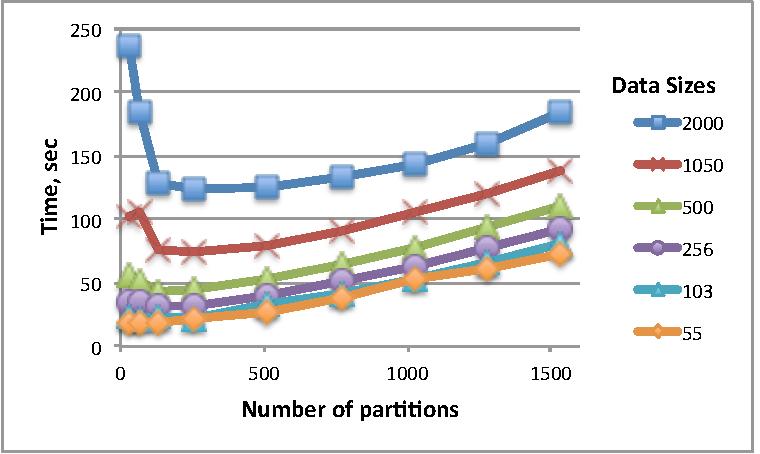
\includegraphics[width=3.2in]{figs/numparts.pdf}
\caption{The number of partitions in the OG data structure TSelect
  query exhibits a bathtub shape - as the number of partitions is
  increased for a given data size, the system performance quickly
  improves, but then starts to deteriorate.  This trend can be seen in
  all data structures.}
\label{fig:numparts}
\end{figure}

\begin{figure}[t!]
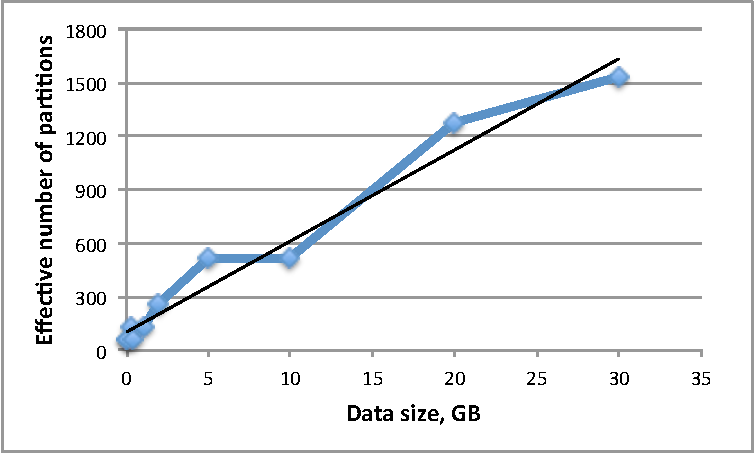
\includegraphics[width=3.2in]{figs/partsfit.pdf}
\caption{There is a linear relationship between data size and the
  optimal number of partitions, as can be seen here with the MG data
  structure.}
\label{fig:partsfit}
\end{figure}

{\bf Outline.}

\reminder{Vera, please write each of these out as \ql queries.  Also
  write what we are keeping fixed in each experiment, and what we are
  varying.}

\begin{enumerate}

\item \insql{TSelect}, to understand the number of
  partitions with which to load for SPG, MG, MGC and OG, as a function
  of data size.

\item \insql{TSelect} + transform (e.g., $a * a$, where $a$ is a
  scalar vertex attribute), to understand the overhead of computing a
  simple transformation operation, with the best settings in
  Experiment 1.  Probably no need for a full experiment,
  let's get a few data points to see whether the overhead is
  noticeable.

\item \insql{TSelect} with \insql{TGroup}, with
  \insql{Any} and \insql{All}.  We will run this experiment for each
  SPG, MG, MGC and OG, with the best setting as determined in
  Experiment 1.  We will then see whether re-partitioning improves
  performance, and will try different partitioning strategies.

\item \insql{TAnd} and \insql{All}, \insql{TOr} with \insql{Any}.  The
  same experiment as Experiment 3.

\item \insql{TSelect} with \insql{pagerank()}. The same
  experiment as Experiment 3.

\item \insql{pagerank()} with \insql{trend()}.  Run only for the best
  data structure of Experiment 5.

\item \insql{TSelect} with \insql{degree()}, only if we have time. The
  same experiment as Experiment 3.

\end{enumerate}
